\documentclass[12pt]{article}
 
\usepackage[margin=1in]{geometry} 
\usepackage{amsmath,amsthm,amssymb}
\usepackage{listings}
\usepackage{graphicx}
\usepackage{float}
\newenvironment{statement}[2][Statement]{\begin{trivlist}
\item[\hskip \labelsep {\bfseries #1}\hskip \labelsep {\bfseries #2.}]}{\end{trivlist}}

\newtheorem{question}{Question}
\newenvironment{answer}{%
  \par\noindent\textbf{Answer:}\quad
}{%
  \hfill$\square$\par
}

\begin{document}
\title{6.8300 Pset 4 Problem 3 writeup} % replace with the problem you are writing up
\author{Zhi Ren} % replace with your name
\maketitle
\section{Positional encoding}
Code written for positional encoding below:
\begin{lstlisting}[language=Python]
    freq_bands = torch.tensor([torch.pi * 2 ** (i+1) 
        for i in range(self.num_octaves)])
\end{lstlisting}


\begin{lstlisting}
# Fill the tensor with sine and cosine embedded values
for i, freq in enumerate(freq_bands):
    embedded_samples[..., i :: 2 * self.num_octaves] 
    = torch.sin(samples * freq)
    # TODO: materize the PE for cos.
    # Copy the below code (a few lines is enough) 
    # to the final submission report.
    # Better to add a small title 
    # "Positional Encoding of NeRF" in the report

    embedded_samples[..., i + 1 :: 2 * self.num_octaves] 
    = torch.cos(samples * freq)    
\end{lstlisting}

\section{NeRF rendering}
There is one line that needs to be filled in in src/nerf.py:
\begin{lstlisting}
# 4. Composite the alpha values and colors
# TODO: call the final composite function
# replace the following line with the final composite function
radiance = self.alpha_composite(alphas, colors)
\end{lstlisting}



\subsection{Short answer question}
\begin{question}
    The rendering model used in our code is slightly different from the one used in the original NeRF paper. Please identify at least one difference.
\end{question}

\begin{answer}
    The rendering model used in our code differs from the one used in the original NeRF paper in that the original paper uses a stratified sampling method to generate samples along the rays, so that they divide the ray into a number of intervals and drawn a random sample from each sinterval, whereas in our code, we take the mid points of all the intervals and there is no random sampling there. 
\end{answer}

\section{Training}
Attached below are several visualizations from the last few iterations of training.
\begin{figure}[H]
    \centering
    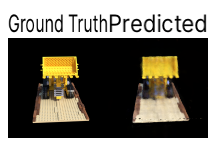
\includegraphics[width=0.8\textwidth]{outputs/progress/007808.png}
    \caption{Visualization of the scene at iteration 7808}
\end{figure}

\begin{figure}[H]
    \centering 
    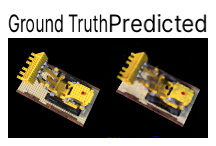
\includegraphics[width=0.8\textwidth]{outputs/progress/007936.png}
    \caption{Visualization of the scene at iteration 7936}
\end{figure}

\begin{figure}[H]
    \centering
    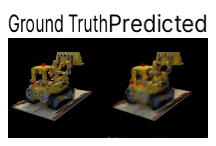
\includegraphics[width=0.8\textwidth]{outputs/progress/008064.png}
    \caption{Visualization of the scene at iteration 8064}
\end{figure}


\section{Final rendering}
From the final rendering: 
\begin{figure}[H]
    \centering
    \begin{minipage}[b]{0.45\linewidth}
        \centering
        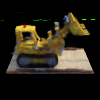
\includegraphics[scale=0.8]{outputs/spin/000000.png}
        \caption{000000 in spin}
        \label{fig:spin000000}
    \end{minipage}\hfill
    \begin{minipage}[b]{0.45\linewidth}
        \centering
        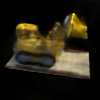
\includegraphics[scale=0.8]{expected_results/000001.png}
        \caption{000001 in spin}
        \label{fig:spin000001}
    \end{minipage}
  \end{figure}







\end{document}